\documentclass[11pt]{article}  
\usepackage{kosemnet,ko-math,ngerman,enumitem}  
\setlist{noitemsep}

\author{Hans-Gert Gräbe, Leipzig}
\title{Reguläre Polyeder\kosemnetlicensemark}
\date{Version vom 25. Oktober 2023}

\begin{document}

\maketitle

\section*{Reguläre Polyeder}

Als \emph{konvexes Polyeder} bezeichnet man einen durch endlich viele ebene
Flä\-chen begrenzten Körper, wo zusammen mit je zwei Punkten auch alle Punkte
der Verbindungsstrecke zu diesem Körper gehören.

Jede Seitenfläche definiert eine Ebene, die \emph{Stützebene} des Polyeders zu
dieser Seitenfläche, so dass das Polyeder vollständig in einem Halbraum
bzgl.\ dieser Ebene liegt. Das Polyeder ist als Punktmenge genau der
Durchschnitt all dieser Halbräume. 

Wir beschränken uns im Weiteren auf beschränkte konvexe Polyeder, das sind
solche mit endlichem Volumen. 

Als \emph{reguläres Polyeder} bezeichnet man ein solches beschränktes konvexes
Polyeder, dessen Seitenflächen alle zueinander kongruente regelmäßige Vielecke
($q$-Ecke) sind \emph{und} in jeder Ecke die gleich Anzahl $p$ von Kanten
zusammenstößt.

Bekanntlich gibt es fünf solche Körper.
\begin{center}
  \includegraphics[width=.8\textwidth]{graebe-05-1/PlatonischeKoerper.jpg}\\
  \emph{Abbildung 1:} Die Platonischen Körper.\\ Quelle: Webseite von
  Carl-Friedrich Bödigheimer, Bonn. 
\end{center}
Dies war bereits in der Antike bekannt, weshalb diese Körper auch als
\textbf{Platonische Körper} bezeichnet werden.  

Dass reguläre Polyeder nur aus regelmäßigen Dreiecken, Vierecken oder
Fünfecken aufgebaut sein können, überlegt man sich zunächst leicht am Aufbau
möglicher Eckenfiguren, siehe Abbildung 2.

\begin{center}
  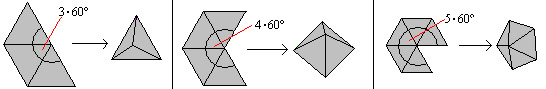
\includegraphics[width=.8\textwidth]{graebe-05-1/winkel-1.jpg}\\
  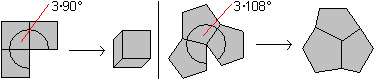
\includegraphics[width=.6\textwidth]{graebe-05-1/winkel-2.jpg}\\
  \emph{Abbildung 2:} Warum nur Dreiecke, Vierecke oder Fünfecke.\\ Quelle:
  Jürgen Köller. Mathematische Basteleien. \cite{KoellerPlatonisch}
\end{center}

Es ist nicht selbstverständlich, aber diese fünf Arten von Eckenfiguren lassen
sich jede zu einem regulären Polyeder zusammensetzen.  Jedes solche regulräe
Polyeder hat eine Umkugel (durch die Ecken), eine Inkugel (diese berührt die
Seitenflächen in deren Zentrum) und eine Kantenkugel (diese berührt die Kanten
in deren Mitten).  Die Kantenkugel ist die Inkugel des Kantengerüsts.

In der folgenden Tabelle sind die Zahl der Ecken $e$, Kanten $k$ und Flächen
$f$ der regulären Polyeder aufgelistet, in denen $p$ regelmäßige $q$-Ecke eine
Eckenfigur bilden.
\begin{center}
  \begin{tabular}{|cc|ccc|l|}\hline
    $p$ & $q$ & $e$ & $k$ & $f$ & Name des Polyeders \\\hline
    3 & 3 &  4 &  6 &  4 & Tetraeder\\
    3 & 4 &  8 & 12 &  6 & Würfel (Hexaeder)\\
    4 & 3 &  6 & 12 &  8 & Oktaeder\\
    3 & 5 & 20 & 30 & 12 & Dodekaeder\\
    5 & 3 & 12 & 30 & 20 & Ikosaeder\\\hline
  \end{tabular}\\[6pt]
  \emph{Tabelle 1:} Kombinatorische Charakteristika der Platonischen Körper
\end{center}

\section*{Einfache Eigenschaften der Platonischen Körper}

\subsection*{Dualität}

$e_W=f_O$ und $e_O=f_W$ ist kein Zufall. Die Mittelpunkte der Seitenflächen
eines Würfels spannen ein Oktaeder auf, die Mittelpunkte der Seitenflächen
eines Oktaeders einen Würfel. Im ersten Fall ist die Inkugel des Würfels die
Umkugel des Oktaeders, die Mittelpunkte $M$ beider Kugeln fallen zusammen.

\begin{minipage}{.5\textwidth}
  Streckt man das Oktaeder mit Zentrum $M$ so, dass die Umkugeln von Oktaeder
  und Würfel zusammenfallen, so durchdringen sich die beiden zueinander dualen
  Polyeder. Genauer: Relevante Kanten schneiden sich in der Mitte und stehen
  senkrecht aufeinander.  Auch die Kantenkugeln beider Polyeder fallen also
  zusammen. Dasselbe gilt für die Inkugeln.

  Ähnlich sind Dodekaeder und Ikosaeder zueinander dual.  Das Tetraeder ist zu
  sich selbst dual.
\end{minipage}\hfill
\begin{minipage}{.4\textwidth}\centering
  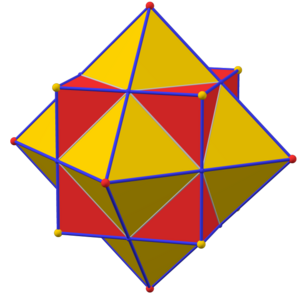
\includegraphics[width=.6\textwidth]{graebe-05-1/Polyhedron_pair_6-8.png}\\
  \emph{Abbildung 3:} Würfel und Oktaeder in dualer Lage. Quelle:
  Wikipedia. 
\end{minipage}

\subsection*{Symmetriegruppen}

Reguläre Polyeder haben eine sehr symmetrische Gestalt und lassen damit viele
räumliche Bewegungen zu, die das Polyeder in sich überführen. Wir wollen alle
herausfinden.  

\textbf{Tetraeder:} Jede der vier Seitenflächen kann nach unten gedreht
werden, und das in jeweils 3 Lagen. Also gibt es 12 Symmetriebewegungen.
Welche?

Dieselbe Frage für die anderen Platonischen Körper.

\subsection*{Größenverhältnisse}

Für jeden der Platonischen Körper fallen die Mittelpunkte von Umkugel,
Kantenkugel und Inkugel zusammen mit dem Zentrum $M$ des Körpers.  Um
Größenverhältnisse zu vergleichen und als Referenz, berechnen wir im Weiteren
die Radien $r_U$ der Umkugel, $r_K$ der Kantenkugel und $r_I$ der Inkugel
sowie Oberfläche $O$ und Volumen $V$ in Abhängigkeit von der Kantenlänge $a$
des jeweiligen Polyeders.  Da sich jedes der regulären Polyeder aus einer
Anzahl kongruenter Pyramiden mit einer der Seitenflächen als Grundfläche und
$M$ als Spitze zusammensetzt, besteht der Zusammenhang $V=\frac13\m O\m r_I$.
Außerdem bestimmen wir die Größe des Winkels zwischen zwei benachbarten
Seitenflächen.

Dabei wollen wir geeignete Schnitte durch die jeweilige räumliche Figur legen,
in denen wir die uns interessierenden Größenverhältnisse in einer ebenen Figur
wiederfinden, und dann Ansätze der ebenen Geometrie zur Anwendung bringen.
  
\paragraph{Tetraeder.}
Lege eine Ebene durch eine Kante und $M$. Diese schneidet die
gegenüberliegende Kante in deren Mitte $K$. Die Schnittfigur ist damit ein
gleichschenkliges Dreieck. Dessen Basis ist eine Kante des Tetraeders der
Länge $a$, die Schenkel sind Höhen in den Seitenflächen der Länge
$h=\frac{a}{2}\sqrt{3}$.  Die Höhen der Länge $H$ auf die Schenkel sind
zugleich die Höhen des Tetraeders und schneiden sich in $M$.  $M$ teilt diese
im Verhältnis $3:1$ (warum?). 

Der untere Abschnitt einer solchen Höhe ist der Berührradius der Inkugel, der
obere Abschnitt der Radius der Umkugel.  Da es eine Bewegung gibt, welche die
beiden gegenüberliegenden Kanten vertauscht, ist $M$ der Mittelpunkt der
dritten Höhe, die die Mitten zweier gegenüberliegender Kanten verbindet, und
deren Länge $h_K$ lässt sich aus $h_K^2=h^2-\br{\frac{a}{2}}^2$ bestimmen.
Daraus ergibt sich $r_K=\frac12\,h_K=\frac{a}{4}\sqrt{2}$.

Auch den Winkel zwischen zwei benachbarten Seitenflächen finden wir in der
ebenen Figur.  Er kann über den Kosinussatz berechnet werden. Aus
$a^2=2h^2(1-\cos(\alpha)$ ergibt sich wegen $2h^2=\frac32\,a^2$
\begin{gather*}
  \cos(\alpha)=1-\frac{a^2}{2h^2}=1-\frac23=\frac13.
\end{gather*}
Zusammengefasst gilt
\begin{itemize}
\item $h=\frac{a}{2}\sqrt{3}$,
\item $H^2=a^2-\br{\frac23\,h}^2=a^2-\frac13\,a^2=\frac23\,a^2$ (Pythagoras),
  also $H=\frac{a}{3}\sqrt{6}$,
\item $r_U=\frac34\,H=\frac{a}{4}\sqrt{6}$,
\item $r_K=\frac{a}{4}\sqrt{2}$, 
\item $r_I=\frac14\,H=\frac{a}{12}\sqrt{6}$,
\item $O=4\m \br{\frac14\sqrt{3}\,a^2}=\sqrt{3}\,a^2$, 
\item $V=\frac13 \br{\frac14\sqrt{3}\,a^2}\m H = \frac{1}{12}\sqrt{2}\,a^3$
  und 
\item $\cos(\alpha)=\frac13$ und damit $\alpha\approx 70.52878\grad$.
\end{itemize}

\paragraph{Würfel.}
Lege eine Ebene durch eine Kante und $M$. Die Schnittfigur ist ein Rechteck
mit den Seitenlängen $a$ und $\sqrt{2}\,a$.  Die Diagonale ist Durchmesser der
Umkugel und hat damit die Länge $2=\sqrt{3}\,a$. Der Winkel zwischen zwei
benachbarten Seitenflächen hat die Größe $\alpha=90\grad$.

Zusammengefasst gilt
\begin{itemize}
\item $r_U=\frac{a}{2}\sqrt{3}$, 
\item $r_K=\frac{a}{2}\sqrt{2}$ (Hälfte der Entfernung zwischen zwei
  gegenüberliegenden Kantenmitten),
\item $r_I=\frac{a}{2}$ (Lot auf die Mitte der Seitenfläche),
\item $O=6\,a^2$,
\item $V=a^3$ und
\item $\cos(\alpha)=0$ wegen $\alpha=90\grad$.
\end{itemize}

\paragraph{Oktaeder.}
Lege eine Ebene durch $M$, eine Ecke $E$ und den Mittelpunkt einer dort
inzidenten Dreiecksfläche. Die Schnittfigur ist eine Raute aus zwei
gleichschenkligen Dreiecken, jedes mit der Basis der Länge $a$ und Schenkeln
der Länge $h=\frac{a}{2}\sqrt{3}$ (Höhe in der Seitenfläche). $M$ ist der
Mittelpunkt der Basis. Die Länge $H$ der Höhe in diesem Dreieck auf die Basis
ergibt sich wieder aus $H^2+\br{\frac{a}{2}}^2=h^2$ zu
$H=r_U=\frac{a}{2}\sqrt{2}$. Das Lot aus $M$ auf den Schenkel trifft diesen im
Schwerpunkt $S$ der Seitenfläche -- das ist zugleich der Berührradius $r_I$
der Inkugel. Es ist also $H^2=\br{\frac23 h}^2+r_I^2$ und damit
$r_I=\frac{a}{6}\sqrt{6}$.  Der Abstand $h_K$ der Mitten gegenüberliegender
Kanten ist gerade gleich $a$ und somit $r_K=\frac{a}{2}$.

Der Winkel zwischen zwei benachbarten Seitenflächen ist gerade der größere der
beiden Innenwinkel der Raute.  Für dessen Größe $\alpha$ ergibt sich nach dem
Kosinussatz $(2H)^2=2h^2(1-\cos(\alpha))$ und damit
\begin{gather*}
  \cos(\alpha)=1-\frac{2H^2}{h^2}=1-\frac{1}{3/4}=1-\frac43=-\frac13.
\end{gather*}
Zusammengefasst gilt
\begin{itemize}
\item $r_U=\frac{a}{2}\sqrt{2}$, 
\item $r_K=\frac{a}{2}$,
\item $r_I=\frac{a}{6}\sqrt{6}$,
\item $O=8\m\frac{a^2}{4}\sqrt{3}=2\sqrt{3}\,a^2$,
\item $V=\frac{a^3}{3}\sqrt{2}$ (als Doppelpyramide mit Höhe $H$) und
\item $\cos(\alpha)=-\frac13$ und damit $\alpha\approx 109.47122\grad$.
\end{itemize}

Untersuchen wir nun die beiden „großen“ Polyeder, das Dodekaeder und das
Ikosaeder. 

\paragraph{Das regelmäßige Fünfeck.}
In beiden Polyedern kommen regelmäßige Fünfecke vor. Als Vorbereitung wollen
wir die Größenverhältnisse in einem solchen regelmäßigen Fünfeck der
Seitenlänge $a$ untersuchen und die Länge $d$ einer der fünf gleich langen
Diagonalen, die Länge $h$ einer der fünf Höhen von einer Ecke auf die
Gegenseite, den Umkreisradius $R$, den Inkreisradius $r$ sowie den
Flächeninhalt $A$ berechnen.

\begin{satz}
  Für ein regelmäßiges Fünfeck mit der Seitenlänge $a$ gilt
  \begin{gather*}
    \begin{array}{cl}    
      \text{\bf Diagonalenlänge:} & d=\frac{a}{2}\,\br{1+\sqrt{5}}\\
      \text{\bf Höhe:} & h=\frac{a}{2}\,\sqrt{5+2\sqrt{5}}\\
      \text{\bf Umkreisradius:} & R=\frac{a}{10}\,\sqrt{50+10\sqrt{5}}\\
      \text{\bf Inkreisradius:} & r=\frac{a}{10}\,\sqrt{25+10\sqrt{5}}\\
      \text{\bf Flächeninhalt:} & A=\frac{a^2}{4}\,\sqrt{25+10\sqrt{5}}
    \end{array}
  \end{gather*}
\end{satz}

\begin{center}
  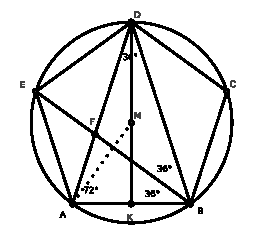
\includegraphics[width=.5\textwidth]{graebe-05-1/Fuenfeck.pdf}\\
  \emph{Abbildung 4:} Größenverhältnisse im Fünfeck
\end{center}

Zeichne im regelmäßigen Fünfeck $ABCDE$ mit Zentrum $M$ die Diagonalen $AD$
und $BE$ ein.  Diese schneiden sich in $F$.  Zeichne weiter die Diagonale $BD$
ein.

Die Dreiecke $ABD$ und $FAB$ sind ähnlich, denn sie sind beide gleichschenklig
mit Basiswinkeln von $72\grad$ und einem Winkel von $36\grad$ an der Spitze.
Weiter ist $BCDF$ eine Raute, da $BC\parallel AD$, $BE\parallel CD$ und
$\msegment{AB}=\msegment{BF}=\msegment{CD}=\msegment{BC}=a$.  Aus der
Ähnlichkeit der beiden Dreiecke folgt $d:a=a:(d-a)$ und damit
\begin{gather*}
  d=\frac{a}{2}\,\br{1+\sqrt{5}}.
\end{gather*}

$h$ kann nun einfach mit Pythagoras im Dreieck $ADK$ berechnet werden, wobei
$K$ die Mitte der Seite $\ksegment{AB}$ ist.  Aus
\begin{gather*}
  h^2+\br{\frac{a}{2}}^2=d^2=\frac{a^2}{2}\br{3+\sqrt{5}}
\end{gather*}
ergibt sich $h=\frac{a}{2}\,\sqrt{5+2\sqrt{5}}$. Auch ist
$h=\frac{a}{2}\tan(72\grad)$, woraus $\tan(72\grad)=\sqrt{5+2\sqrt{5}}$ folgt.

Ähnlich kann eine Formel für den Radius $R=\msegment{AM}$ aufgestellt werden.
Im rechtwinkligen Dreieck $AKM$ ergibt sich
\begin{gather*}
  R^2=\br{\frac{a}{2}}^2+(h-R)^2,
  \intertext{daraus}
  2\,h\,R=\br{\frac{a}{2}}^2+h^2=\frac{a^2}{4}\,\br{6+2\sqrt{5}}
  \intertext{und weiter}
  R=\frac{a}{4}\,\frac{6+2\sqrt{5}}{\sqrt{5+2\sqrt{5}}}
  =\frac{a}{2}\,\frac{\br{3+\sqrt{5}}\sqrt{5-2\sqrt{5}}}{\sqrt{5^2-20}}
  =\frac{a}{2}\,\frac{\sqrt{10+2\sqrt{5}}}{\sqrt{5}} =
  \frac{a}{10}\,\sqrt{50+10\sqrt{5}}, 
\end{gather*}
wobei im vorletzten Schritt 
\begin{gather*}
  \br{3+\sqrt{5}}\sqrt{5-2\sqrt{5}} =\sqrt{\br{3+\sqrt{5}}^2\br{5-2\sqrt{5}}}
  =\sqrt{10+2\sqrt{5}}
\end{gather*}
ausmultipliziert wurde.

$r=\msegment{MK}=h-R$ ist der Inkreisradius, für den wir aus derselben
Beziehung nun
\begin{align*}
  r^2&=R^2-\frac{a^2}{4} =\frac{a^2}{100}\,\br{50+10\sqrt{5}}-\frac{a^2}{4}
  =\frac{a^2}{100}\,\br{25+10\sqrt{5}}
\end{align*}
erhalten. Es folgt $r=\frac{a}{10}\sqrt{25+10\sqrt{5}}$.

Der Flächeninhalt $A$ setzt sich aus fünf gleichschenkligen Dreiecken mit
Grundseite $a$ und Spitze $M$ zusammen. Es ergibt sich
\begin{gather*}
  A=5\m\frac{a}{2}\,r =\frac{a^2}{4}\,\br{25+10\sqrt{5}}.
\end{gather*}

Wegen $\frac{r}{R}=\sin(54\grad)$ im selben Dreieck $AKM$ ergibt sich auch
noch 
\begin{gather*}
  \sin(54\grad)=\frac{\sqrt{25+10\sqrt{5}}}{\sqrt{50+10\sqrt{5}}}
  =\frac{\sqrt{750+250\sqrt{5}}}{\sqrt{50^2-500}}
  =\frac{5\sqrt{30+10\sqrt{5}}}{20\sqrt{5}}
  =\frac{1}{4}\sqrt{6+2\sqrt{5}}
\end{gather*}
wobei im zweiten Schritt mit $50-10\sqrt{5}$ erweitert und
$\br{25+10\sqrt{5}}\br{50-10\sqrt{5}}=750+250\sqrt{5}$ zusammengefasst wurde.
Dieser Ausdruck kann weiter vereinfacht werden, denn es ist
$\sqrt{6+2\sqrt{5}}=1+\sqrt{5}$, wie man unmittelbar nachrechnet.  Damit haben
wir $\sin(54\grad)=\frac{\sqrt{5}+1}{4}$.

Solche Vereinfachungen geschachtelter Wurzelausdrücke können systematisch mit
folgendem Satz gefunden werden:  

\begin{satz}
  Es ist $\sqrt{a+2\sqrt{b}}=\sqrt{c}+\sqrt{d}$ mit positiven ganzen Zahlen
  $a,b,c,d$ ($b$ kein volles Quadrat) genau dann, wenn $x^2-ax+b=(x-c)(x-d)$
  gilt.
\end{satz}

\begin{beweis}
  Quadrieren von $\sqrt{a+2\sqrt{b}}=\sqrt{c}+\sqrt{d}$ zeigt, dass $a=c+d,
  b=c\m d$ zumindest eine hinreichende Bedingung für die Gültigkeit der
  Beziehung ist.  Ist $\sqrt{b}$ irrational, so ist sie auch notwendig.
\end{beweis}

\paragraph{Dodekaeder und Ikosaeder.}
Wir kommen zu Dodekaeder und Ikosaeder zurück und erzeugen eine Schnittfigur
durch die Ebene, die durch einen Eckpunkt, den Durchmesser durch diesen
Eckpunkt (und damit durch das Zentrum $M$ des Körpers) und eine dazu adjazente
Kante bestimmt ist.  Für beide Körper entsteht als Schnittfigur ein Sechseck
$E_1E_2K_3E_4E_5K_1$, wobei $E_{1\dots4}$ Ecken und $K_{1,3}$ Mitten
gegenüberliegender Kanten des jeweiligen Polyeders sind.  Dann ist
$r_U=\msegment{ME_1}$.  Weiter ist $K_2$ die Mitten der Seite
$\ksegment{E_1E_2}$ und damit $r_K=\msegment{MK_1}$.  $\ksegment{E_1K_1}$
verbindet Ecke und gegenüberliegende Kantenmitte einer Seitenfläche. Auf
dieser Strecke liegt auch der Mittelpunkt $F_1$ dieser Seitenfläche, für den
$r_I=\msegment{MF_1}$ ist. $\kangle{E_1K_1E_4}$ ist dann der Winkel zwischen
zwei Seitenflächen. 

\begin{center}
  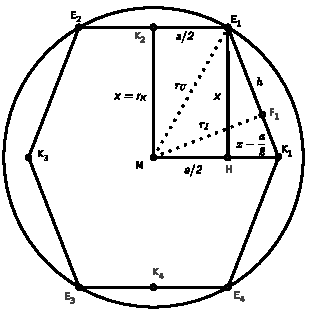
\includegraphics[width=.5\textwidth]{graebe-05-1/Schnittfigur.pdf}\\
  \emph{Abbildung 5:} Die Schnittfigur, nach \cite{Fendt1}
\end{center}

Die Rechnungen hierfür sind in \cite{Fendt1, Fendt2} ausgeführt.  Zunächst
wird $x=r_K$ aus der Beziehung 
\begin{gather*}
  x^2+\br{x-\frac{a}{2}}^2=h^2
\end{gather*}
berechnet, die sich im Dreieck $E_1HK_1$ ergibt, wobei $H$ der Lotfußpunkt aus
$E_1$ auf $MK_1$ ist.  $h$ ist dabei die Höhe einer Seitenfläche, also eines
gleichseitigen Dreiecks (Ikosaeder) oder eines regelmäßigen Fünfecks
(Dodekaeder).  Dann wird $r_U$ im Dreieck $ME_1K_2$ aus
\begin{gather*}
  x^2+\br{\frac{a}{2}}^2=r_U^2
\end{gather*}
berechnet.  Schließlich wird $r_I$ im Dreieck $MF_1E_1$ aus
\begin{gather*}
  r_U^2=r_I^2+y^2
\end{gather*}
berechnet, wobei $y=\msegment{E_1F_1}$ der obere Abschnitt der Höhe einer
Seitenfläche und damit gleich deren Umkreisradius ist.  Die Größe der
Oberfläche $O$ ergibt sich unmittelbar aus Vervielfachung der entsprechenden
Inhaltsformel für eine Seitenfläche, das Volumen $V$ aus der Summe der
Volumina der Pyramiden über den Seitenflächen mit Spitze in $M$ zu
$V=\frac13\m O\m r_I$.  Für die Größe $\alpha$ des Winkels
$\kangle{E_1K_1E_4}$ zwischen zwei Seitenflächen erhalten wir schließlich
wieder mit dem Kosinussatz $(2x)^2=2h^2(1-\cos(\alpha))$ und daraus
$\cos(\alpha)=1-\frac{2x^2}{h^2}$.  

Dies liefert für das Dodekaeder mit der Seitenlänge $a$
\begin{itemize}
\item $r_U=\msegment{ME_1}=\frac{a}{4}\,\sqrt{3}\br{1+\sqrt{5}}$ für den
  Umkugelradius,
\item $r_K=\msegment{MK_3}=\frac{a}{4}\br{3+\sqrt{5}}$ für den
  Kantenkugelradius,
\item $r_I=\msegment{MF_1}=\frac{a}{20}\,\sqrt{250+110\sqrt{5}}$ für den
  Inkugelradius,
\item $O=12\m A=12\m\frac{a^2}{4}\,\sqrt{25+10\sqrt{5}}
  =3\,a^2\,\sqrt{25+10\sqrt{5}}$,
\item $V=12\m\frac13\,A\,r =\frac{a^3}{4}\,\br{15+7\sqrt{5}}$ (12 Pyramiden
  auf den Seitenflächen mit Spitze im Zentrum des Polyeders) und
\item $\cos(\alpha)=-\frac15\sqrt{5}$ und damit $\alpha\approx
  116.56505\grad$.
\end{itemize}
und für das Ikosaeder
\begin{itemize}
\item $r_U=\msegment{ME_1}=\frac{a}{4}\,\sqrt{10+2\sqrt{5}}$ für den
  Umkugelradius,
\item $r_K=\msegment{MK_3}=\frac{a}{4}\br{1+\sqrt{5}}$ für den
  Kantenkugelradius,
\item $r_I=\msegment{MF_1}=\frac{a}{12}\,\br{3\sqrt{3}+\sqrt{15}}$ für den
  Inkugelradius,
\item $O=5\,a^2\,\sqrt{3}$,
\item $V=\frac{5}{12}\,a^3\,\br{3+\sqrt{5}}$ und
\item $\cos(\alpha)=-\frac13\sqrt{5}$ und damit $\alpha\approx
  138.18969\grad$.
\end{itemize}

\paragraph{Kugelähnlichkeit der regulären Polyeder.}
Untersuchen wir zum Schluss, wie „nahe“ die einzelnen regulären Polyeder einer
Kugel kommen.  Wir wollen dabei drei Größen vergleichen, und zwar
\begin{gather*}
  K_1=\frac{O}{4\pi r_U^2},\ K_2=\frac{V}{\frac43\pi
    r_U^3}\ \text{und}\ K_3=\frac{r_I}{r_U}.
\end{gather*}
$K_1$ bestimmt, wie nahe die Oberfläche des Polyeders der Oberfläche seiner
Umkugel kommt, $K_2$ bestimmt dasselbe für das Volumen und $K_3$ sagt etwas
über die „Abweichung“ von der Form einer Sphäre aus.

Brefeld betrachtet in \cite{Brefeld} als weiteren Parameter $K_4$ die
\emph{Sphärizität} (siehe dazu auch \cite{Sphaer}) als Quotient aus der
Oberfläche einer Kugel gleichen Volumens und der Oberfläche des jeweiligen
Polyeders.  Dazu ist für das entsprechende Polyeder mit der Seitenlänge $a$
aus dessen Volumenformel $V(a)$ zunächst der Radius einer solchen Kugel
gleichen Volumens über die Volumenformel $V(a)=\frac{4\pi}{3}r(a)^3$ zu
bestimmen und dieser Ausdruck dann in die Formel $O=4\pi r^2$ für die
Oberfläche der Kugel einzusetzen.
\begin{gather*}
  K_4=\frac{\sqrt[3]{36\pi\m V(a)^2}}{O(a)}
\end{gather*}
\newpage

Aus den oben berechneten Werten ergeben sich die folgenden Formeln und
Näherungswerte:

\begin{center}\small
  \begin{tabular}{|l|c|c|c|c|}\hline
    & $K_1$ & $K_2$ & $K_3$ & $K_4$\\\hline

    \rule[-16pt]{0pt}{30pt}Tetraeder & $\frac{2}{\sqrt{3}\pi}\approx 0.368$ &
    $\frac{2}{3\sqrt{3}\pi}\approx 0.123$ & $\frac13\approx 0.333$ &
    $\sqrt[3]{\frac{\pi}{6\sqrt{3}}}\approx 0.671$\\
    
    \rule[-16pt]{0pt}{16pt}Würfel & $\frac{2}{\pi}\approx 0.637$ &
    $\frac{2}{\sqrt{3}\pi}\approx 0.368$ & $\frac{1}{\sqrt{3}}\approx 0.577$ &
    $\sqrt[3]{\frac{\pi}{6}}\approx 0.806$\\

    \rule[-16pt]{0pt}{16pt}Oktaeder & $\frac{\sqrt{3}}{\pi}\approx 0.551$ &
    $\frac{1}{\pi}\approx 0.318$ & $\frac{1}{\sqrt{3}}\approx 0.577$ &
    $\sqrt[3]{\frac{\pi}{3\sqrt{3}}}\approx 0.846$\\
    
    \rule[-16pt]{0pt}{16pt}Dodekaeder &
    $\frac{2\sqrt{25+10\sqrt{5}}}{(3+\sqrt{5})\pi}\approx 0.837$ &
    $\frac{5+\sqrt{5}}{\sqrt{3}\pi}\approx 0.665$ &
    $\frac{250+110\sqrt{5}}{5\sqrt{3}(1+\sqrt{5})}\approx 0.795$ &
    $K_4(D)\approx 0.910$\\
    
    \rule[-16pt]{0pt}{16pt}Ikosaeder &
    $\frac{10\sqrt{3}}{(5+\sqrt(5)\pi}\approx 0.762$ &
    $\frac{5+\sqrt{5}}{\sqrt{10+2\sqrt{5}}\pi}\approx 0.605$ &
    $\frac{3+\sqrt{5}}{\sqrt{3}\sqrt{10+2\sqrt{5}}}\approx 0.795$ & $
    \sqrt[3]{\frac{(7+3\sqrt{5})\pi}{30\sqrt{3}}}\approx 0.939 $\\\hline
  \end{tabular}\\[6pt]
  \emph{Tabelle 2:} Parameter der Kugelähnlichkeit der Platonischen Körper
\end{center}

Auch für $K_4(D)$ lässt sich ein exakter Wurzelausdruck mit einem CAS berechnen:
\begin{gather*}
  K_4(D)=\sqrt[3]{\frac{(47+21\sqrt{5})\pi}{(30+12\sqrt{5})\sqrt{25+10\sqrt{5}}}}. 
\end{gather*}
In \cite{Sphaer} wird für diesen Ausdruck eine andere Formel angegeben.  Auch
wenn die näherungsweise Berechnung nahe legt, dass beide Formeln dieselbe
reelle Zahl beschreiben, ist es mühevoll, dies exakt nachzuweisen.

\section*{Der Eulersche Polyedersatz}

Wir haben die fünf Platonischen Körper intensiver untersucht, allerdings
bleibt noch ein kleiner Zweifel, ob es nicht doch noch andere reguläre
Polyeder gibt.  Irgendwie ist zwar klar, dass das nicht sein kann, da wir ja
für jedes mögliche Paar $(p,q)$ eine Bauvorschift angeben können -- nimm
genügend viele kongruente reguläre $q$-Ecke, baue $p$ von ihnen zu einer
Eckenfigur zusammen und klebe die restlichen Schritt für Schritt an, bis der
Körper fertig ist.  Überraschend ist eher, dass das in jedem Fall gelingt,
sich die Konstruktion also zu einem Polyeder schließt, und nicht die mögliche
Mehrdeutigkeit. 

\emph{Euler} hat einen Zusammenhang zwischen den Anzahlen der Ecken $e$,
Kanten $k$ und Seitenflächen $f$ gefunden, der für alle konvexen Polyeder gilt
und es gestattet, für die Platonischen Körper diese Anzahlen zu berechnen,
ohne zu wissen, wie sie aussehen.

\begin{satz}[Polyedersatz, Euler 1758]
Hat ein konvexes Polyeder $e$ Ecken, $k$ Kanten und $f$ Seitenflächen,
so gilt stets \[e-k+f=2\,.\]
\end{satz}

\emph{Beweisskizze}: Es gibt verschiedene Beweise dieses Satzes. Eine
besonders elementare Über\-legung verwendet das schrittweise
``Aufschneiden'' in ein ebenes Körpernetz und untersucht, wie sich
dabei die Zahlen $e,k,f$ und $Z=e-k+f$ verändern. Wir bezeichnen die
neuen Werte jeweils mit $e',k',f',Z'$.

Zunächst wird eine Seitenfläche herausgeschnitten: $e'=e, k'=k,
f'=f-1$, also $Z'=Z-1$.

Danach werden weitere Kanten aufgeschnitten, bis das Körpernetz
schließlich ausgebreitet werden kann. Bei jedem Schnitt wird es eine
Ecke und eine Kante mehr: $e'=e+1, k'=k+1, f'=f, Z'=Z$.

Das Körpernetz ist ein ebener (überschneidungsfreier) Graph mit Ecken
und Kanten. Die Seitenflächen nennen wir jetzt ``Gebiete''.  Nun
werden in diesem Netz nacheinander die inneren Kanten entfernt:
\begin{itemize}
\item[(1)] Trennt die innere Kante zwei Gebiete, so werden diese beiden
  Gebiete vereinigt: $e'=e, k'=k-1, f'=f-1, Z'=Z$.
\item [(2)] ``Hängt'' die innere Kante nur noch an einer Ecke und ragt
  in ein Gebiet hinein, so wird beim Entfernen der Kante die Anzahl
  der Gebiete nicht geändert. Die Kante verschwindet zusammen mit dem
  an ihr ``hängenden'' Eckpunkt: $e'=e-1,k'=k-1,f'=f, Z'=Z$.
\end{itemize}
Schließlich bleibt nur noch ein einziges Gebiet übrig, das von $n$
Ecken und dann logischerweise auch $n$ Kanten begrenzt wird, die einen
Ring bilden $e=k=n, f=Z=1$. $\Box$\medskip

\subsection*{Anwendung der Eulerschen Polyedersatzes}

Der Eulersche Polyedersatz kann verwendet werden, um die Anzahlen der Ecken
$e$, Kanten $k$ und Seitenflächen $f$ der regulären Polyeder durch rein
kombinatorische Rechnungen zu bestimmen, ohne deren genaue Form zu kennen.

Wie oben bestehe das reguläre Polyeder aus regelmäßigen $q$-Ecken als
Seitenflächen und in jeder Ecke stoßen die gleich Anzahl $p$ von Kanten (und
damit auch Seitenflächen) zusammen.

Dann ist $p\cdot e$ die Summe der von den Ecken ausgehenden Kanten. Dabei
haben wir die Kanten allerdings doppelt gezählt, denn jede Kante hat zwei
Endpunkte: $2\,k = p\cdot e$. Genauso bekommen wir $2\,k = q\cdot f$, wenn wir
die Anzahlen der Kanten aller Flächen aufsummieren, da jede Kante an zwei
Flächen angrenzt. Aus der Eulerformel $e-k+f=2$ folgt 
\[\frac{1}{p} + \frac{1}{q} =  \frac12 +\frac{1}{k}. \tag{G}\]
Wegen $p,q\ge 3$ muss $p,q<6$ gelten, denn sonst wäre $\frac{1}{p} +
\frac{1}{q} \le \frac12$.  Die Gleichung (G) hat deshalb genau die fünf
bereits eingangs in Tabelle~1 aufgelisteten Lösungen.

\subsection*{Das Fußballpolyeder}

Kann man auch aus anderen gleichartigen Eckenfiguren Polyeder zusammenbauen?
Eine solche Konstruktion mit größtmöglicher Kugelähnlichkeit ergibt sich, wenn
in einer Ecke zwei Sechsecke und ein Fünfeck zusammenstoßen.  Diese
Konstruktion ist als Fußball weithin bekannt. Wir wollen abschließend den
Eulerschen Polyedersatz auf diese Situation anwenden.

Das Fußballpolyeder hat $e$ Ecken, $k$ Kanten und $f=f_5+f_6$ Seitenflächen,
wobei $f_5$ die Zahl der Fünfecke und $f_6$ die Zahl der Sechsecke bezeichnet.
In jeder Ecke stoßen drei Kanten zusammen: $3\,e=2\,k$.  Vergleichen wir
Kanten und Seitenflächen, so ergibt sich wie oben $2\,k=5\,f_5+6\,f_6$.

Die Eckenfiguren lassen sich höchstens so zusammenbauen, dass jedes Fünfeck
von 5 Sechsecken umgeben und jedes Sechseck von drei Fünfecken und drei
Sechsecken umgeben ist.  $3\,f_6=5\,f_5$: Zählen wir alle Kontakte zwischen
Fünf- und Sechsecken, so haben wir jedes Fünfecke fünfmal und jedes Sechseck
dreimal gezählt.  Wir erhalten $f_6=\frac53\,f_5$, $e=\frac23\,k$ und
$2\,k=5\,f_5+6\,f_6=15\,f_5$, also $f_5=\frac{2}{15}\,k$,
$f_6=\frac53\,f_5=\frac{2}{9}\,k$ und damit aus dem Eulerschen Polyedersatz
\begin{gather*}
  2=e-k+f=\frac23\,k-k+\frac{2}{15}\,k+\frac{2}{9}\,k=\frac{1}{45}\,k
\end{gather*}
und damit $k=90$, $e=60$, $f_5=12$, $f_6=20$. 


\begin{thebibliography}{xxx}
\bibitem{Brefeld} Werner Brefeld (1999-2023). Platonische Körper und
  archimedische Körper.\\
  \url{http://www.brefeld.homepage.t-online.de/polyeder.html} (25.10.2023) 
\bibitem{Fendt1} Walter Fendt (2005). Das Dodekaeder.\\
  \url{https://www.walter-fendt.de/math/geo/dodekaeder.pdf} (12.10.2021) 
\bibitem{Fendt2} Walter Fendt (2005). Das Ikosaeder.\\
  \url{https://www.walter-fendt.de/math/geo/ikosaeder.pdf} (12.10.2021) 
\bibitem{KoellerPlatonisch} Jürgen Köller. Mathematische Basteleien.
  Platonische Körper.\\
  \url{http://www.mathematische-basteleien.de/platonisch.htm} (10.10.2021)
\bibitem{KoellerFuenfeck} Jürgen Köller. Mathematische Basteleien.
  Regelmäßiges Fünfeck.\\
  \url{http://www.mathematische-basteleien.de/fuenfeck.htm} (10.10.2021)
\bibitem{Wikipedia} Wikipedia. Platonische Körper.\\ 
  \url{https://de.wikipedia.org/wiki/Platonischer_K%C3%B6rper} (10.10.2021)
\bibitem{Sphaer} Wikipedia. Sphärizität (Geologie).\\ 
  \url{https://de.wikipedia.org/wiki/Sph%C3%A4rizit%C3%A4t_(Geologie)}\\
    (27.10.2023)
\end{thebibliography}

\begin{attribution}
graebe (2005-07-24): Eine erste Version dieses Material (Eulerscher
Polyedersatz) wurde für die Projektarbeit in Klasse 11/12 fürs Mathelager 2005
in Ilmenau erstellt und dort auch eingesetzt.

graebe (2021-10-13): Modifiziert für einen Workshop über 60 Minuten für Klasse
13 in der Inspirata\footnote{\url{https://www.inspirata.de/}}.  Es wurden
Platonische Körper aus Klickmaterial zusammengebaut, Ecken, Kanten, Flächen
gezählt, invariante Drehbewegungen analysiert und zum Schluss der Eulersche
Polyedersatz bewiesen sowie kurz auf das Fußballpolyeder eingegangen.

graebe (2023-10-10): Zwei kleine Fehler berichtigt.

graebe (2023-10-27): Überarbeitung für einen Vortrag in der
LSGM-Herbstschule. 
\end{attribution}

\end{document}

Aufbereitet für Maxima: [T,W,O,D,I]
ru:[sqrt(6)/4,sqrt(3)/2,1/sqrt(2),sqrt(3)/4*(1+sqrt(5)),1/4*sqrt(10+2*sqrt(5))];
ri:[sqrt(6)/12,1/2,1/sqrt(6),1/20*sqrt(250+110*sqrt(5)),1/12*sqrt(3)*(3+sqrt(5))];
O:[sqrt(3),6,2*sqrt(3),3*sqrt(25+10*sqrt(5)),5*sqrt(3)]*a^2;
V:[sqrt(2)/12,1,sqrt(2)/3,1/4*(15+7*sqrt(5)),5/12*(3+sqrt(5))]*a^3;

K1(i):=O[i]/(4*%pi*ru[i]^2);
K2(i):=V[i]/(4/3*%pi*ru[i]^3);
K3(i):=ri[i]/ru[i];
K4(i):=(36*V[i]^2*%pi)^(1/3)/O[i]; 
